\vspace{-0.3cm}
\section{Wafer-Scale GEMV}\label{sec:gemv}
\vspace{-0.2cm}

In this section, we describe \gemv, a scalable GEMV algorithm for PLMR devices.

\subsection{PLMR compliance in distributed GEMV}

\begin{figure}[t!]
    \centering
    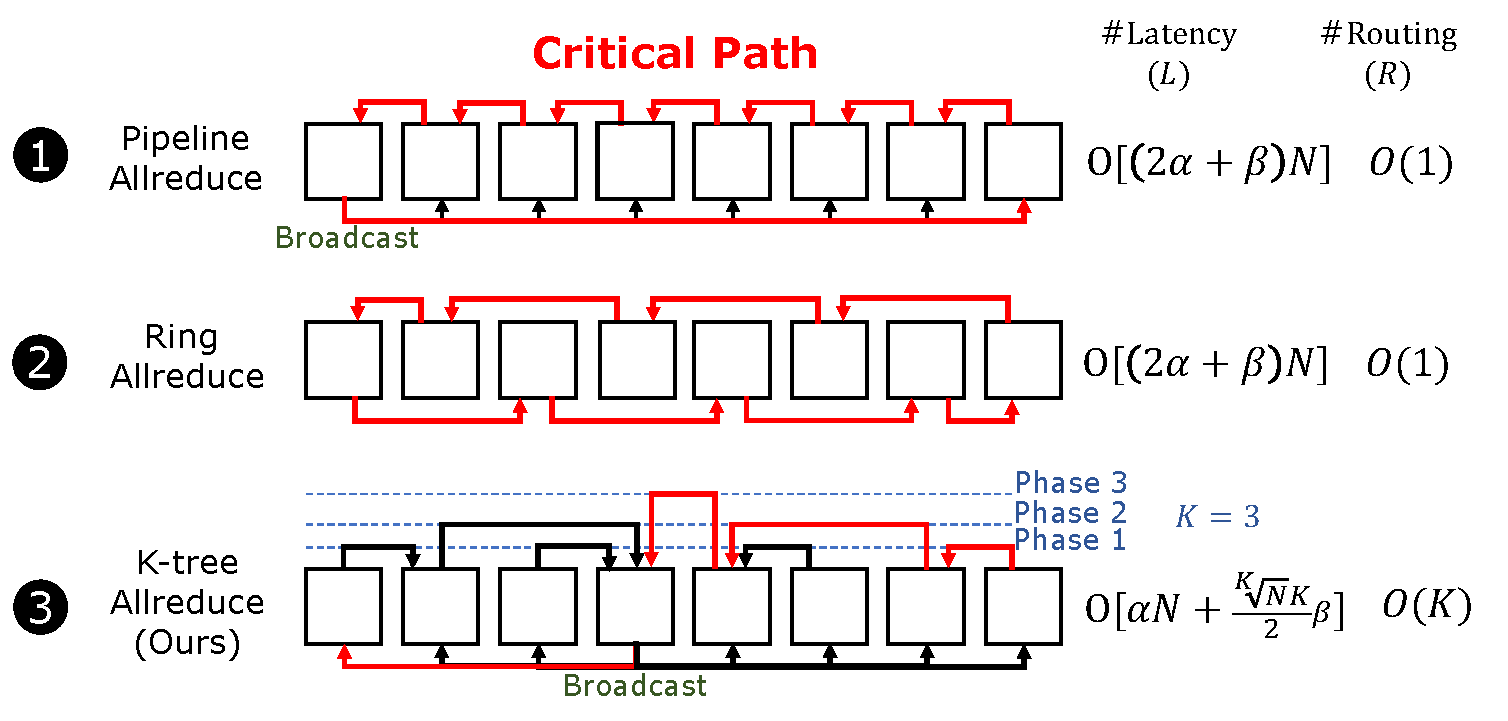
\includegraphics[width=1\linewidth]{imgs/reduce-algo.pdf}
    \caption{PLMR compliance in distributed GEMV}
    \label{fig:gemv-plmr-compliance}
\end{figure}

The completion time of a distributed GEMV is primarily determined by an element-wise computation to generate a partial sum result at each core and then an allreduce operation that aggregates partial results from all selected cores and then sends the aggregated results back to all cores for the continuous GEMV. As the analysis in GEMM, in wafer-scale GEMV, we also define the following metrics: 
(i)~\emph{Routing paths per core}: The number of routing paths per core, with fewer paths ensuring compliance with the R property
(ii)~\emph{Latency of critical path}: Maximal latency of the whole allreduce communication, mainly determined by the time from when the partial sum is sent from the farthest core to when the aggregated sum is received by the farthest core.

We analyze current distributed GEMV methods and show how \gemv meets these metrics:

\begin{enumerate}[label=(\arabic*), leftmargin=0.5cm, noitemsep,topsep=0pt]

 \item \textbf{GEMV with pipeline allreduce} is commonly used in TPU pod systems~\cite{google2023efficiently} and as the default in Cerebras demo~\cite{cerebrasgemv}. As illustrated by the red line in the Figure \ref{fig:gemv-plmr-compliance}~\circled{1}, the critical path of the pipelined all-reduce starts from the farthest core, where partial sums are reduced step-by-step toward the root core, and the aggregated result is then broadcast from root to all cores. While this approach ensures that the routing path per core remains within the $R$ constraint, $O(1)$ per-core routing resource usage, it incurs a total of $2N$ hops and $N$ routing stages, violating the L property.

\item \textbf{GEMV with ring allreduce} is commonly used in GPU pod systems, where it is the default configuration, especially for a large amount of data \cite{wafer-reduce}. As shown by \circled{2} in Figure~\ref{fig:gemv-plmr-compliance}, the critical path of ring allreduce involves each partial sum traversing all cores in the ring. Similar to pipelined allreduce, this approach maintains $O(1)$ routing paths per core, but incurs a communication latency of $O\left[(2\alpha + \beta)N\right]$, thus violating the latency constraint $L$ defined in PLMR.

\item \textbf{GEMV with K-tree allreduce (Ours)}. As analyzed above for pipelined and ring allreduce, the sequential execution of reduce-add operations leads to $N$ routing stages along the critical path. In contrast, K-tree allreduce organizes the reduce-add path as a balanced K-tree, enabling $K$ phases grouped parallel reductions with $O(\sqrt[K]{N})$ cores per group and reducing the critical path to only $\frac{\sqrt[K]{N}K}{2}$ times routing and $N$ hops. However, this comes at the cost of requiring $O(K)$ routing paths per core.

\end{enumerate}

\vspace{-3mm}
\subsection{The \gemv algorithm}
\vspace{-1mm}

We will outline the key steps of \gemm below:

\begin{enumerate}[label=(\arabic*), leftmargin=0.5cm, noitemsep,topsep=0pt]
\item \textbf{Initialization:} Consider $C = A \times B$ and $A$ is a vector. \gemv will partition $B$ into tiles $B_{sub}$ along two dimensions, forming $N \times N$ tiles and distributed across the cores. For $A$, \gemv will partition it along the vector length, forming $N$ tiles distributed on one axis and replica $A$ on another axis. Each core receives one tile of $A_{sub}$ and one of $B_{sub}$. Then we determine which cores form a group to obtain aggregated results in each phase based on the K-tree.

\item \textbf{Parallel computation:} In this stage, each core performs a local GEMV $A_{\text{sub}} \times B_{\text{sub}}$ to obtain $C_{sub}$ partial sum.

\item \textbf{Aggregation:} The aggregation step primarily involves using the K-tree allreduce we design. The key steps are as follows: (i)~In the 1st-phase, each group performs group reduction and obtains the partial sum of $C_{sub}$ at the root core of each group. (ii)~In the $k$th-phase, the results from the $(k-1)$~th-phase are reduced to the root cores of each group in the $k$th-phase. After K times repeating, $C$ can be obtained by concatenating the $C_{sub}$ from all K-tree root cores. (iii)~Optionally, a broadcast operation from the root core of the $K$-tree may follow, depending on whether continuous GEMV is required.
\end{enumerate}

\mypar{Scalability Analysis}  
As shown in \circled{3} of Figure~\ref{fig:gemv-plmr-compliance}, this method scales efficiently with parallelism and meets the L property by selecting an appropriate $K$. It requires $K+1$ paths at the tree root core but allows flexible adjustment of $K$ to address R based on hardware limitations. Compared to pipeline and ring all-reduce, K-tree all-reduce essentially builds pass-through paths between distant cores by consuming routing resources, thereby reducing routing latency.

However, a larger $K$ is not always better, as it depends on $N$ and R constraints. Additionally, larger $K$ increases routing complexity and overhead. Considering these factors, we have chosen $K=2$ for our current implementation, evaluated in the following sections.